%%%%%%%%%%%%%%%%%%%%%%%%%%%%%%%%%%%%%%%%%%%%%%%%%%%%%%%%%%%%%%%%%%%%%%%%%%%%%%%%%%%%%%%%%%%%
\chapter{Statique des fluides}
\section{Équations générales}
Au cours des précédents chapitre, nous avions obtenus quatre \textit{équations générales} :
\begin{equation}
	\left\{\begin{array}{ll}
	\text{Équation de continuité : } & \frac{\partial \rho}{\partial t} + \partial_i(\rho v_i)
	=0\\
	\text{Équation d'équilibre : } & \tau_{ij,j} + f_i = 0\\
	\text{Loi de comportement : } & \tau_{ij} = -p\delta_{ij}\\
	\text{Équation d'état : } & F(\rho,p, \theta) = 0
	\end{array}\right.
\end{equation}
Sans faire plus d'hypothèse, en combinant l'équation d'équilibre avec la loi de comportement,
on trouve :
\begin{equation}
	-\frac{\partial p}{\partial x_j}\delta_{ij} + f_i = 0\ \ \ \ \ \text{ou }\ \ \ 
	\frac{\partial p}{\partial x_i} = f_i
\end{equation}
Pour atteindre un équilibre, les forces de volume ne peuvent pas être quelconques :
\begin{equation}
	\vec{f} = \overline{grad}\ p \Leftrightarrow \overline{rot}\ \vec{f} = \vec{0}
\end{equation}

\subsection{Force massique}
Reprenons la définition des forces par unité de masse : $\vec{f}dV = \vec{F}dm = \vec{F}
\rho dV$, ce qui peut s'écrire $f_i = \rho F_i$. La condition $\overline{rot}\ \vec{f} =
\vec{0}$ s'écrit :
\begin{equation}
	\overline{rot}\ (\rho\vec{F}) = \vec{0}\ \ \ \ \ \text{ou }\ \ \ \delta_{ijk}\partial_j
	(\rho F_k) = 0
\end{equation}
Par les propriétés du rotationnel, on peut également obtenir
\begin{equation}
	\overline{grad}\ \rho \times \vec{F} + \rho\,\overline{rot}\ \vec{F} = \vec{0}
\end{equation}		
	
	
	
\subsection{Force dérivant d'un potentiel}
Lorsque les forces massiques dépendent d'un potentiel, on retrouve l'expression tant
convoitée d'\textit{Analyse I, Physique générale, Mécanique rationnelle I,...} à 
savoir $\vec{F} = -\overline{grad}\ U \rightarrow \overline{rot}\ \vec{F} = \vec 0$.\\
Cette condition implique 
\begin{equation}
	\vec{F}\times \overline{grad}\ \rho = 0
\end{equation}
Cela signifie que les surfaces $\rho = C^{ste}$ sont des surfaces $U = C^{ste}$.
Dans le cas de la pesanteur, les valeurs de $U$ constantes sont des plans horizontaux
où la valeur de $\rho$ est constante.\\
	
Les équation d'équilibres:
\begin{equation}
	\left\{\begin{array}{ll}
	\vec{f} &= \overline{grad}\ p\\
	\vec{F} &= -\overline{grad}\ U
	\end{array}\right.
\end{equation}
donnent
\begin{equation}
	\rho\vec{F} = \overline{grad}\ p\ \ \ \Rightarrow\ \ -\rho\,\overline{grad}\ U =
	\overline{grad}\ p
\end{equation}
Cette nouvelle implication nous permet de conclure que :
\begin{itemize}
	\item les surfaces $U = C^{ste}$ sont des surfaces $p = C^{ste}$.
	\item les surfaces $\rho = C^{ste}$ sont des surfaces $U = C^{ste}$.
\end{itemize}
Avec l'équation d'état $F(\rho,p,\theta) = 0$, on obtient 
\begin{equation}	
	\left\{\begin{array}{ll}
	p &= p(U)\\
	\rho &= \rho(U)\\
	\theta &= \theta(U)
	\end{array}\right.
\end{equation}
Compte-tenu des deux conclusions énoncées ci-dessus, $p(U)$ 
donne $\partial_i p = \frac{dp}{dU}\partial_i U$ ou encore $\overline{grad}\ p = 
\frac{dp}{dU}\overline{grad}\ U$. Cette nouvelle relation permet de définir $\rho(
U)$ :
\begin{equation}
	\left\{\begin{array}{ll}
	\overline{grad}\ p &= \frac{dp}{dU}\,\overline{grad}\ U\\
	-\rho\,\overline{grad}\ U &= 	\overline{grad}\ p
	\end{array}\right.\ \ \ \ \ \Rightarrow \rho = -\dfrac{dp}{dU}
\end{equation}


\subsection{Définition de la fonction $P$}
Les équations d'équlibres puvent s'écrire sous la forme de deux gradients :
\begin{equation}
	\grad U + \dfrac{1}{\rho}\ \grad p = 0
\end{equation}
Supposons pouvoir définir une fonction $P$ telle que
\begin{equation}
	\grad P = \dfrac{1}{\rho}\ \grad p\ \ \ ou\ \ \ \partial_iP = \dfrac{1}{\rho}
	\partial_i p
\end{equation}
Les équations d'équlibres s'écrivent alors :
\begin{equation}
	\grad P + \grad U = 0
\end{equation}
ou encore $P + U = C^{ste}$.
	
	
%%%%%%%%%%%%%%%%%%%%%%%%%%%%%%%%%%%%%%%%%%%%%%%%%%%%%%%%%%%%%%%%%%%%%%%%%%%%%%%%%%%%%%%%%%%%
\section{Principe d'Archimède}
\subsection{Énoncé}
L'origine du problème vient du calcul de la résultante des forces de pression exercée par
un fluide sur un corps immergé en équilibre ; même si la distribution de pression est 
connue, avec la forme géométrique de la surface $S$ compliquée, bonne chance pour 
calculer 
\begin{equation}
	\vec{A} = \oint \overline{T}^{(n)}\ dS = \oint -p\ \vec{n}\ dS
\end{equation}
Pour régler le problème, on définit un postulat : \textit{l'équilibre du fluide n'est 
pas changé si on remplace le corps immergé par du fluide}. L'équilibre de volume $V$ 
du fluide s'écrit alors :
\begin{equation}
	\underbrace{\int_V (-\rho\ g)\vec{1_z}\ dV}_{1} + \underbrace{\oint_S (-p)\vec{n}\ dS
		=0}_{2}
\end{equation}
\begin{enumerate}
	\item Poids du fluide remplaçant le corps immergé
	\item Postulat : on a gardé la distribution de pression inchangée
\end{enumerate}
Comme $\vec A = \oint - p\vec{n}\ dS$, en faisant passer l'autre terme de l'autre côté
de l'égalité, après inversion du signe on trouve 
\begin{equation}
	\vec{A} = \int_V (\rho\ g)\vec{1_z}\ dV
\end{equation}
Ce qui n'est rien d'autre que l'action du fluide sur le corps immergé, soit la poussée
d'Archimède qui est une force :
\begin{itemize}
	\item Dirigée vers le  haut.
	\item De module égale au poids de fluide déplacé.
	\item Appliqué au centre de masse de ce fluide : le centre de poussée.
\end{itemize}
	
\textbf{Attention !} Il ne faut pas baisser sa garde et garder en têtes deux choses:
\begin{enumerate}
	\item La poussée d'Archimède traduit $\oint_S (-p)\vec{n}\ dS$, il ne faut donc pas 
	      appliquer la poussée d'Archimède \textbf{et} la résultante des pressions !
	\item Ce principe ne s'applique \textbf{pas} si l'équilibre est modifié !
\end{enumerate}    
    
\subsubsection{Le ballon}
Un exemple d'application du principe, slide 15-17
	    
\subsubsection{Le bateau}
Un exemple réel, slide 22
	    

\section{Équilibre des fluides incompressibles}
\subsection{Fluides homogènes}
Un fluide incompressible - petit rappel - ne l'est que si le volume qu'il occupe
ne change pas de mesure au cours du temps, c'est à dire : $\rho^\bullet = 0$. Par 
ailleurs, le fluide est dit homogène si $\rho = \rho_0$\footnote{L'huile remonte 
	à la surface de l'eau ; dépendance en $x \rightarrow$ non homohène.}. La 
définition de $P$ 	devient :
\begin{equation}
	\overline{grad}\ P = \frac{1}{\rho_0}\ \grad p
\end{equation}
ou encore $P = \frac{p}{\rho_0}$. Les équations d'équilibres deviennent
\begin{equation}
	\grad (U + P) = 0\ \ \ \ \ \text{ou }\ \ \ U + \frac{p}{\rho_0} = C^{ste}
\end{equation}
	
Considérons comme potentiel la pesanteur $U = gz$. Les équations d'équilibre se
modifient facilement:
\begin{equation}
	gz + \frac{p}{\rho_0} = C^{ste}\ \ \ \ \ \text{ou }\ \ \ p+\rho_0gz = C^{ste}
\end{equation}
\begin{center}
	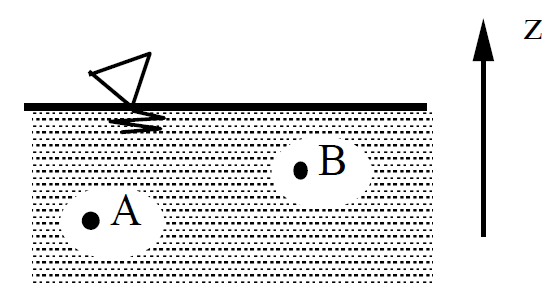
\includegraphics[scale=0.3]{ch7/1}
	\captionof{figure}{Equilibre des fluides incompressibles}
\end{center}
	
Considérons deux points $A$ et $B$ à une coordonée de hauteur respectivement 
$z_a$ et $z_b$\footnote{Simple application de $p+\rho_0gz = C^{ste}$.} :
\begin{equation}
	p_a +\rho_0 gz_a = p_b +\rho_0gz_b
\end{equation}
Il suffit d'un point ou la pression est connue pour founir la valeur de la 
constante. Notons que la surface libre d'un liquide (où la pression est 
constante) pesant est horizontale.
	
\subsubsection{Exemple 1 : les vases communicants}
\begin{center}
	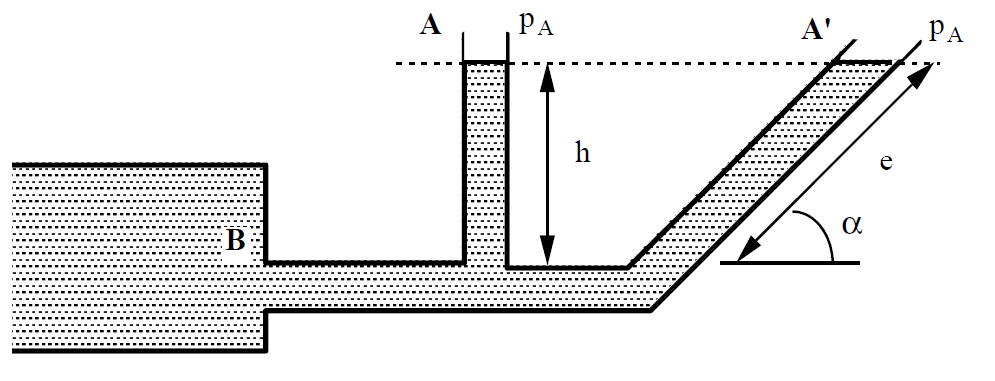
\includegraphics[scale=0.3]{ch7/2}
	\captionof{figure}{Les vases communicants}
\end{center}
Le principe est de mesurer une différence de pression  en mesurant une 
différence de hauteur liquide : la différence de niveau $z_a-z_b$ permet 
de calculer la différence de pression.
\begin{equation}
	p_b-p_a = \rho_0g(z_a-z_b)
\end{equation}
Si comme ici le tuyau est incliné, c'est toujours au même $z_a$ que l'on 
se réfère.
		
\subsubsection{Exemple 2 : répartition des pressions sur une paroi}
Si ici $p+\rho_0gz = C^{ste}$, c'est parce que nous sommes face à un 
gradient. Le niveau de référence peut être fixé librement : $z=0$ à la 
surface et tant qu'on y est $p=0$.\\
\begin{center}
	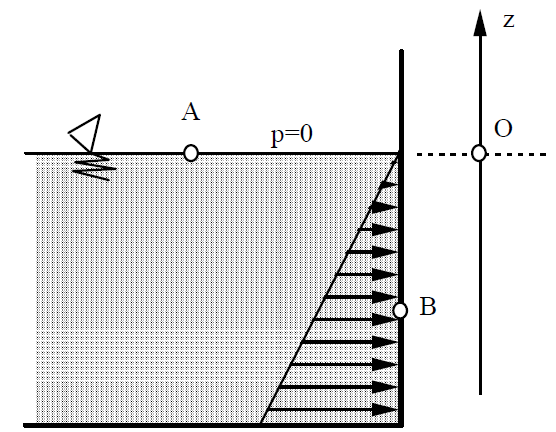
\includegraphics[scale = 0.4]{ch7/3}
	\captionof{figure}{Répartition des pressions sur une parois}
\end{center}
 		
Considérons un point $A$ de la surface libre (car $p$ et $z$ est connu en ce
point) ainsi qu'un point $A$ d'une certaine "altitude" $z$. En écrivant la loi :
\begin{equation}
	\underbrace{p_A}_{=0} + \underbrace{\rho_0gz_A}_{z_A=0} = \underbrace{p_B}_{?} +
	\underbrace{\rho_0gz_B}_{z_B=z}
\end{equation}				
On trouve alors $p=-\rho_0gz$. \textbf{Attention !} Les pressions agissent 
perpendiculairement aux parois, il ne faut pas se tromper lors des représentations!
				
		
\subsection{Le principe de Pascal}
\textit{Si en un point $A$ d'un fluide incompressible homogène, la pression est 
	accrue de $\Delta p$, tous les points du fluide subissent le même accroissement de 
	pression $\Delta p$.}   
